\block{Description du Système}{
 	{ \fontsize{40}{40}\selectfont 
 	
	Le système construit est composé de plusieurs étapes.

    \vspace{1em}
    \begin{center}
        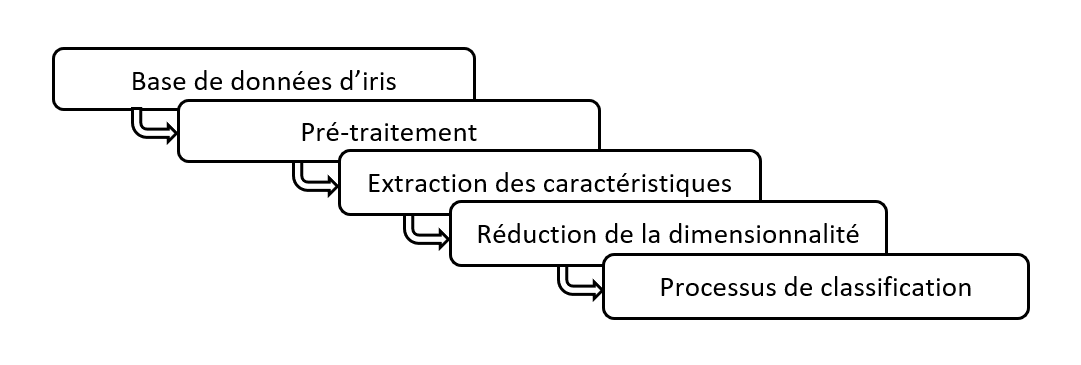
\includegraphics[width=0.9\linewidth]{schema}
        \captionof{figure}{Schéma du système.}
    \end{center}
    \vspace{1em}
    
    \section{Base de données}
    La base de donéees utilisée pour ce projet est « MMU iris dataset ».Elle est composée d’images d’oeil pour l’entraînement de modèles de système biométrique basé sur l’iris
de l’oeil. Cet ensemble de données se compose de 5 images de l’iris gauche et droit de
46 personnes.

	\section{Pré-traitement}
	
	\section{Extraction des caractéristiques}
	
	\section{Réduction de la dimensionnalité}
	
	\section{Processus de classification}
    
	}
}

\block{Évaluation}{
 	{ \fontsize{40}{40}\selectfont 
 	
	Texte ... 
	
	}
}